\documentclass{article}

\usepackage{amsmath}
\usepackage{amssymb}
\usepackage{parskip}
\usepackage{fullpage}
\usepackage{hyperref}
\usepackage{tikz}
\usepackage{wrapfig}
\usepackage{bettelini}

\hypersetup{
    colorlinks=true,
    linkcolor=black,
    urlcolor=blue,
    pdftitle={Integration},
    pdfpagemode=FullScreen,
}

\title{Integration}
\author{Paolo Bettelini}
\date{}

\begin{document}

\maketitle
\tableofcontents
\pagebreak

\section{Indefinite Integrals}

\subsection{Definition}

Given a function \(f(x)\), an \textbf{anti-derivative} or \textbf{primitive}
is any function \(F(x)\) such that
\[
    \frac{dF}{dx} = f(x)
\]
The operator to find a primitive function is called the \textbf{indefinite integral}
\[
    \integral[f(x)][x]=F(x)+C,
    \quad C\in\mathbb{R}
\]
The function to integrate (integrand) is delimited by the integral symbol \(\int\)
and a differential of the variable of integration \(dx\).
\\
A function has infinitely many primitives, hence the \(+ C\) term. This essentially
means that the derivative of a function is the same when the function is shifted
up or down, the rate of change is the same. By reversing the process we don't know
the up or down shift of the original function.
\[
    f(x)=\integral[\frac{df}{dx}][x] + C
\]
for some specific \(C\).

\subsection{Properties}

If \(k\) is a constant
\[
    \integral[kf(x)][x] = k \integral[f(x)][x]
\]

\[
    \integral[f(x) \pm g(x)][x] = \integral[f(x)][x] \pm \integral[g(x)][x]
\]

\subsection{Substitution Rule}

Given an integral in the form
\[
    \integral[f(g(x))g'(x)][x]
\]
Let
\[
    u = g(x)
\]
The differential of u is then
\[
    du=g'(x)dx
\]
meaning that we can rewrite the integral as
\[
    \integral[f(u)][u] = F(u) + C = F(g(x)) + C
\]

\pagebreak

\subsection{Integration By Parts}

Starting from the product rule
\[
    \frac{d}{dx}\big(f(x)g(x)\big)=f'(x)g(x)+f(x)g'(x)
\]
if we integrate both parts we get
\begin{align*}
    f(x)g(x)+C&=\int f'(x)g(x)\,dx+\int f(x)g'(x)\,dx \\
    \int f(x)g'(x)\,dx &= f(x)g(x)+C - \int f'(x)g(x)\,dx 
\end{align*}
Since the indefinite integral of \(f'(x)g(x)\) is equal to some function plus an arbitrary constant, we can ignore the \(+C\) term.
\[
    \int f(x)g'(x)\,dx = f(x)g(x) - \int f'(x)g(x)\,dx
\]

\pagebreak

\section{Definite Integrals}

\subsection{Area Problem}

\begin{wrapfigure}{l}{10cm}
    \begin{center}
        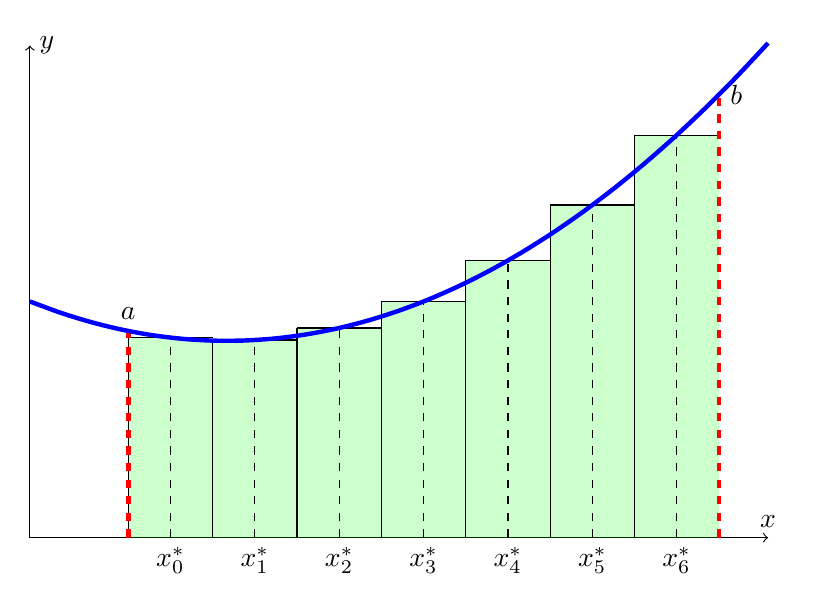
\begin{tikzpicture}[
            scale=1.25,
            declare function={
                func(\x) = 0.1 * (\x - 2) * (\x - 2) + 2;
                Width=7.5;
                Height=5;
                A = 1;
                B = 7;
                N = 7;
                Delta = {(B-A) / N};
            }
        ]
            \draw[->] (0, 0) -- (0, Height) node[right] {\(y\)};
            \draw[->] (0, 0) -- (Width, 0) node[above] {\(x\)};
    
            \pgfmathtruncatemacro\END{N-1}
            \foreach \x in {0,1,...,\END} {
                % rectangle
                \fill [green, opacity=0.2]
                    ({A + Delta * \x}, 0) rectangle ({A + Delta * (\x+1)}, {func(A + Delta * (\x + 0.5))});
                
                \draw[-] ({A + Delta * \x}, 0)
                    -- ({A + Delta * \x}, {func(A + Delta * (\x + 0.5))});

                \draw[-, dashed] ({A + Delta * (\x + 0.5)}, 0)
                    node[below] {\(x_{\x}^*\)}
                    -- ({A + Delta * (\x + 0.5)}, {func(A + Delta * (\x + 0.5))});

                % line over rectangle
                \draw[-] ({A + Delta * \x}, {func(A + Delta * (\x + 0.5))})
                    -- ({A + Delta * (\x+1)}, {func(A + Delta * (\x + 0.5))});
            }
    
            \draw[-, dashed, red, ultra thick] (A, 0) -- (A, {func(A)}) node[above, black] {\(a\)};
            \draw[-, dashed, red, ultra thick] (B, 0) -- (B, {func(B)}) node[right, black] {\(b\)};
    
            \draw[domain=0:Width, smooth, variable=\x, blue, ultra thick] plot ({\x}, {func(\x)});
        \end{tikzpicture}
    \end{center}
\end{wrapfigure}

We want to find the signed area between \(f(x)\) and the \(x\)-axis between
the interval \([a;b]\).\\
One way to do it would be by dividing the area into \(n\) rectangles, each of width
\[
    \Delta x = \frac{b-a}{n}
\]
The height of each triangle is given by \(f(x_k^*)\).
The area under the curve is approximately
\[
    A \approx \sum_{k=0}^{n-1}f(x_k^*)\Delta x
\]
Notice that the position of \(x_k^*\) within the base of each rectangle controls the type of
the approximation of the area under the curve.
By moving \(x_k^*\) within the base we may achieve an approximation by abundance
or defect.
The type of approximation does not matter when we let \(n\to \infty\).
As the amount of rectangles approaches infinity, the approximation approaches
the exact value of the area.
\[
    A = \lim_{n\to\infty} \sum_{k=0}^{n}f(x_k^*)\Delta x
\]

\subsection{Definition}

Given a function \(f(x)\) continuous on the interval \([a;b]\), we divide the interval
into \(n\) rectangles of width \(\Delta x = \frac{b-a}{n}\) and height \(f(x_k^*)\).
The definitive interval of \(f(x)\) from \(a\) to \(b\) is
\[
    \integral[a][b][f(x)][x] = \lim_{n\to \infty} \sum_{k=0}^{n} f(x_k^*)\Delta x
\]

\subsection{Properties}

\[
    \integral[a][b][f(x)][x] = -\integral[b][a][f(x)][x]
\]
If \(k\) is constant
\[
    \integral[a][b][cf(x)][x] = c\integral[a][b][f(x)][x]
\]
\[
    \integral[a][b][f(x)\pm g(x)][x] = \integral[a][b][f(x)][x] \pm \integral[a][b][g(x)][x]
\]
\[
    \integral[a][a][f(x)][x] = 0
\]

\subsection{Fundamental Theorem of Calculus}

If \(f(x)\) is continuous on \(I=[a;b]\),
\[
    g(x) \integral[a][x][f(t)][t]
\]
is also continuous on \(I\) and
\[
    g'(x)=f(x)
\]
or in other words
\[
    \frac{d}{dx}\integral[a][x]f(t)[t]=f(x)
\]

\end{document}
